There are patterns we readily recognize as ordered, and there are phenomena that appear disordered at first sight. The distinction is not a property of nature so much as a description we impose to make sense of what we observe. Crucially, attending to what seems disordered has often yielded the deepest insights. Apparent irregularity can be a sign that our current descriptions are incomplete rather than that the world itself is incoherent.

Take the planets. To the ancient eye, most stars traced regular paths across the heavens, but a handful—the planētai, or “wanderers”—appeared to deviate. They sometimes slowed, looped backward in retrograde, and resumed their forward motion. This was not ignored: Greek and later Ptolemaic astronomers developed elaborate schemes of epicycles that reproduced these motions and gave real predictive power. Yet the irregularities remained troubling, because they clashed with the philosophical ideal of uniform circular motion thought to govern the heavens. For centuries, the wandering of the planets embodied a residual disorder within an otherwise orderly cosmos. In the late 1500s, Tycho Brahe’s meticulous positional measurements sharpened the discrepancy: planetary motions deviated systematically from circular models, even with refinements. In 1609, Johannes Kepler drew a different boundary. By proposing that planetary orbits were ellipses rather than circles, he preserved predictive accuracy while dissolving the irregularities into a new kind of order—the apparent disorder of retrograde motion was reinterpreted as the natural projection of elliptical orbits onto the sky.

A similar story unfolded three centuries later. In 1827, the Scottish botanist Robert Brown observed pollen grains suspended in water dancing with a jitter that seemed erratic and, in his words, “life-like.” No known physical law explained this motion, and for decades it remained an emblem of disorder at the microscopic scale. In 1905, Albert Einstein reframed the problem. Drawing on the molecular-kinetic theory of heat, he proposed that the jitter was not purposeless noise but the statistical consequence of innumerable collisions with unseen water molecules~\cite{UberMolekularkinetischenTheorie}. Importantly, he did not render each trajectory predictable; rather, he showed that the ensemble followed precise statistical laws. In 1908, Jean Perrin confirmed this experimentally by tracking particles under a high-power microscope and comparing their distributions to Einstein’s predictions~\cite{r.BrownianMovementMolecular1911}. His careful measurements provided direct evidence for the discrete, molecular nature of matter, earning him the Nobel Prize in 1926.

These historical episodes remind us that what we call “disorder” is often a structure we have not yet resolved—and that the path toward understanding is driven by two fundamental forces. First, the drive to look closer: to improve our ability to observe what was previously invisible, by increasing the accuracy and precision of experimental measurements. Second, the drive to think differently: to reinterpret what we observe, forming new theoretical models that both explain current data and forecast the system’s behavior. These two forces often work in tandem: new perspectives inspire the invention of new tools, and new tools reveal patterns that force a change in perspective. This offers a lens that is both optimistic and humbling: optimistic, because even apparent disorder may yield new insight when studied carefully; humbling, because each advance in understanding often uncovers further layers of the unknown.

\section{Defects in crystalline materials}
Turning the clock forward to modern times, we find similar storylines. In modern condensed matter physics, one of the most ordered systems is the crystal lattice, or its physical realization-- crystalline solid. A crystal lattice is a repeating two or three-dimensional arrangement of atoms or molecules; by knowing the smallest repeating building block- the unit cell, and the translational symmetry it follows, one can reconstruct the whole crystal lattice. However, in real crystalline solids, defects are always present, and the perfect order is almost never followed. Defects are any localized structures that break the local translational symmetry in a crystal. The name 'Defect' accurately points out its disordered nature in a highly ordered system; it is also a negative-sounding word (as being defective) that reflects the undesirable attitude people used to hold towards it. At the beginning of the twentieth century, condensed matter physicists wished to explain the intrinsic properties of the materials with the newly developed tools and concepts in quantum mechanics. At that time, the focus was purely defect-free periodic crystals, and it is unclear even to the brightest minds then, what positive role defects might play \cite{lorentzVortrageUberKinetische1914} \cite{spitalerPerspectivesTheoryDefects2018}. The first recorded work about defects was in Pierre Curie's seminar paper on the thermal transport properties of solids \cite{ZurKinetischenTheorie}, where Curie discussed the qualitative influence of these 'lattice perturbations' on the flow of heat and electricity. However, when Curie drafted a manuscript on this topic, he received strong resistance from Wolfgang Pauli, a leading figure in quantum mechanics and by then, a member of Pierre's phD committee. Pauli disregarded the study around defects by commenting: "the residual resistivity is caused by dirt and one should not dwell in dirt"(\textit{ist der Restwiderstand ein Dreckeffect und im Dreck soll man nicht wühlen}). It is shocking to see that a subject matter is argued as unworthy of studying, especially from the mouth of one of the fathers of modern physics. The arrogance and prejudice towards the study of defects were unprecedented at the time.

The tone shifted with the study on semiconductors and their applications in World War II. One the one hand, due to the urgent need for purer Germanium(Ge) and Silicon(Si) in Radar detection, new growth and material purification techniques were developed; on the other hand, controlling and engineering the electronic properties of Ge and Si becomes important; one way is to introduce atoms from a different column of the periodic table to replace the host atoms. These alien atoms disrupt the lattice periodicity and are considered impurities. However, since these impurities have different charge states and can donate either positive charge carriers(holes) or negative charge carriers(electrons) to the parent system, they are labeled as 'dopants' to differentiate from those undesirable impurities. Although the studies around dopants were still preliminary during the war, they demonstrated the defect's potential to manipulate materials and shifted the initial undignified narrative towards defect study within the scientific community.

This narrative shift gave birth to several decades of study of defects, especially in semiconductors like Si, and the rewards are tremendous. By controlling the density and spatial distribution of different dopants, scientists were granted the power to engineer the asymmetry of the carrier flow. This superpower formed the backbone of the third industrial revolution from the mid-twentieth century; it bears the invention of transistors and diodes, which led to the microprocessor and integrated circuit, the foundations of modern computing and digital devices.   

Another area where defect studies have profoundly shaped our understanding is in metals and metallic alloys. The most notable case is steel, an alloy of iron and carbon. While the use of iron and steel tools dates back to around 1200 BC, modern scientific investigation into their properties only took off in the early twentieth century. In the 1920s and 1930s, a major puzzle emerged: the experimentally measured stiffness and yield strength of metals were orders of magnitude lower than theoretical predictions. For instance, in copper (Cu), theory predicted an ideal shear strength of about 5 GPa \cite{frenkelZurTheorieElastizitaetsgrenze1926}, yet annealed Cu yielded at only 0.5–5 MPa—a gap of roughly a thousandfold. This discrepancy was resolved in 1934, when Egon Orowan, Michael Polanyi, and G. I. Taylor independently proposed that plastic deformation could be explained by the motion of dislocations—linear crystalline defects. Under shear stress, a half-plane of atoms can shift by breaking and reforming bonds along a dislocation line, one (or a few) at a time, rather than breaking all the bonds across an entire plane simultaneously. This mechanism requires far less energy than moving the plane in unison.

The ability to “look closer” was also a key element. Advances such as X-ray diffraction, transmission electron microscopy, and later atom probe tomography allowed scientists to directly observe dislocations, grain boundaries, precipitates, and segregation at the atomic scale \cite{50YearsTEM}\cite{guoSegregationdislocationSelforganizedStructures2025}\cite{AtomProbeTomography}. In the 21st century, these tools—combined with in-situ mechanical testing, synchrotron and neutron diffraction, and high-fidelity computational modeling—have made it possible to link specific defect characteristics to macroscopic mechanical behavior in steels \cite{liReviewRecentProgress2022}\cite{kimSituNeutronDiffraction2020}\cite{gadalinskaDirectDeterminationPhase2021}. Modern defect engineering now controls dislocation density, tunes nanoscale precipitates, and manipulates grain boundary character to achieve targeted combinations of strength, ductility, toughness, and fatigue resistance. This precision has enabled unprecedented alloy design: as of August 2025, the Register of European Steels lists over 3,500 grades of steel, with the majority developed in the 21st century.

The transformation of our understanding about defects in classical materials like metals and semiconductors allowed us to create and engineer materials to meet our needs, which fathered the modernization and digitization of this era; these experiences and knowledge also set the stage for another even richer frontier: defects in quantum materials. On this end, the study of defects is not only about improving materials, but it is about uncovering new physics. 

\section{Defect study in quantum materials}
Quantum material is a community-adopted umbrella term rather than a sharply defined scientific term like 'conductor' or 'insulator'. Commonly, it refers to a solid-state system whose macroscopic behavior is dominated by quantum many-body effects and/or topological quantum states, often leading to emergent phenomena absent in classical materials. Unlike noble metals, p–n semiconductors, and other classical systems well described by single-electron band theory, quantum materials deviate sharply from this picture:
\begin{itemize}
	\item \textbf{Strongly correlated electron systems} break the independent-electron approximation because Coulomb repulsion rivals or exceeds kinetic energy\cite{hubbardElectronCorrelationsNarrow1963}; this can generate entirely new orders, such as the insulating state of a half-filled Mott insulator like V2O3, where theory predicts a metal\cite{mcwhanMottTransitionCrDoped1969}\cite{mottMetalInsulatorTransition1968}\cite{mottMetalInsulatorTransitions1990}.
	\item \textbf{Unconventional superconductors} depart from the conventional BCS framework, with pairing symmetries and mechanisms rooted in electronic correlations rather than phonons\cite{OutShadowBCS2006}; in cuprates like 
	YBa\textsubscript{2}Cu\textsubscript{3}O\textsubscript{7$-\delta$}, this leads to d-wave superconductivity\cite{tsueiPairingSymmetryFlux1994}\cite{hardyPrecisionMeasurementsTemperature1993}\cite{kirtleySymmetryOrderParameter1995}.
	\item \textbf{Topological materials} exhibit electronic structures defined by global topological invariants, producing robust boundary states immune to weak disorder\cite{chiuClassificationTopologicalQuantum2016}; in Bi\textsubscript{2}Se\text{3}, this manifests as spin-polarized surface states protected by time-reversal symmetry\cite{panElectronicStructureTopological2011}\cite{jozwiakSpinpolarizedSurfaceResonances2016}\cite{sobotaUltrafastElectronDynamics2014}.
\end{itemize}
Beyond these, heavy Fermion systems host quasiparticles with effective masses hundreds of times that of free electrons\cite{wirthExploringHeavyFermions2016}\cite{stewartHeavyfermionSystems1984}. Low-dimensional and moiré systems, such as magic-angle twisted bilayer graphene, amplify quantum effects through geometry\cite{caoUnconventionalSuperconductivityMagicangle2018}\cite{carrTwistronicsManipulatingElectronic2017}, while quantum spin systems, including Kitaev magnets, host long-range entanglement and fractionalized excitations\cite{normanHerbertsmithiteSearchQuantum2016}\cite{banejeeNeutronScatteringProximate2017}—phenomena far beyond the reach of classical band theory.  

Compared to classical systems, quantum materials exhibit an amplified sensitivity to disorder. This is partly because their emergent orders typically stabilize only at low ordering temperatures, often in the range of a few to tens of kelvins(~100 K in the case of cuprate superconductors), far below the characteristic energy scales of classical magnets or structural transitions. At such low energies, even subtle perturbations from impurities, vacancies, or strain can compete directly with the ordering tendencies.

A vivid example comes from the hole-doped cuprate superconductors, which present intertwined orders across different phase space\cite{fradkinIntertwinedOrdersPhysics2025}. Figure \ref {fig:cuprate_pd} shows their temperature–doping phase diagram. It is defined by a prominent superconducting dome, flanked on the underdoped side by an antiferromagnetic Mott insulating state and an extended pseudogap regime, and on the overdoped side by a correlated metallic state. As doping is tuned toward the dome edges, for instance near $p=p_c$ at low temperature, the system approaches quantum critical points (QCPs) where the balance between intertwined orders is exquisitely delicate. Here, the introduction of even a small concentration of defects—such as cation substitution or oxygen nonstoichiometry—can shift transition temperatures, reshape phase boundaries, or suppress one order in favor of another.

This heightened susceptibility is not confined to cuprates. In frustrated quantum magnets, low ordering temperatures mean that a few percent of nonmagnetic site dilution can melt long-range order and stabilize spin-liquid-like ground states\cite{syzranovEffectVacancyDefects2022}. In heavy fermion materials, weak disorder can cause drastic phase shifts at sub-kelvin scales\cite{toldinDisorderQuasiparticleInterference2013}\cite{gegenwartQuantumCriticalityHeavyfermion2008}, and induce metallic behavior in Kondo insulators \cite{pirieVisualizingAtomicscaleOrigin2023}. Topological materials require a nuanced addendum: bulk topological invariants confer robustness of extended states to weak local disorder, yet defects (from point defects to dislocations/disclinations) can host bound modes that are invisible to bulk averages but informative in local probes. 

As emphasized in Millis’ classification of disorder effects in correlated systems\cite{millisClassificationEffectsDisorder2003}, such fragility is a double-edged sword—degrading desired properties in some contexts while providing a uniquely sensitive lever for probing the interplay of various quantum orders. This reflects two unique opportunities that the defect study offers. First, mapping defect structure and formation pathways can directly inform synthesis protocols and help uncover the intrinsic properties. A topical case is the actinide superconductor UTe\textsubscript{2}, where people were initially puzzled as experimental results of this system show significant variations. It was shown later that crystal quality is the key factor behind these discrepancies, after a series of studies on disorder in UTe\textsubscript{2} enabled by advanced growth methods\cite{aishwaryaMeltingChargeDensity2024}\cite{xueAdvancesSingleCrystal2025}. Secondly, defects can be leveraged as tunable knobs and probes: By purposefully introducing disorder like chemical substitutions, vacancies, or irradiation, one can interrogate couplings among subtle orders\cite{fradkinIntertwinedOrdersPhysics2025}\cite{ohDisentanglingIntertwinedOrders2025}.   

\begin{figure} 
	\centering
	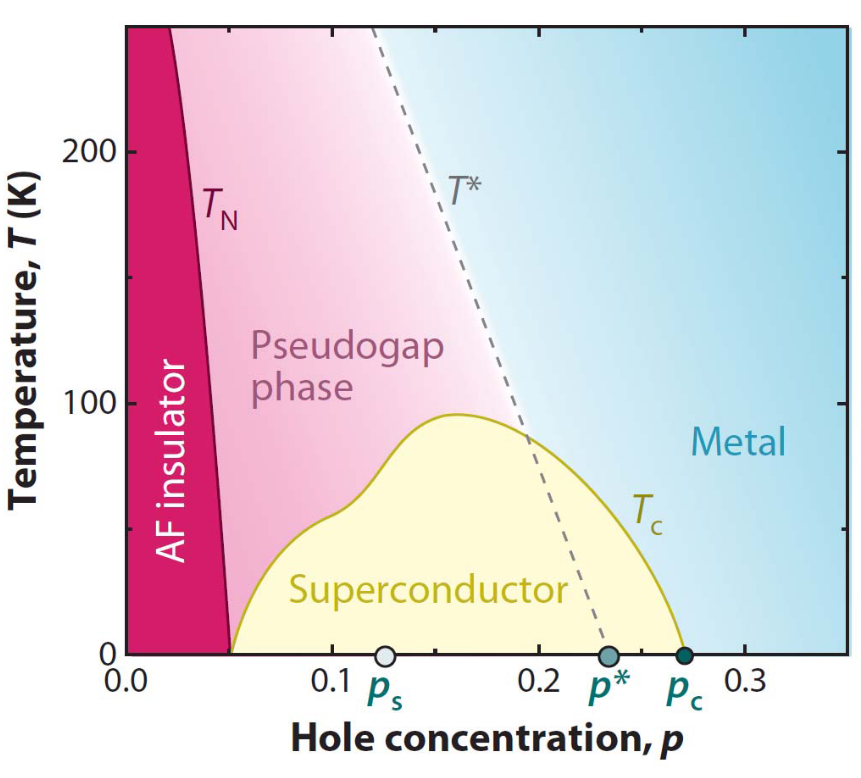
\includegraphics[width=\textwidth]{Cuprate_phasediagram.png}
	\caption[\textbf{A sketch of the phase diagram of cuprate superconductor}]{\textbf{A sketch of the phase diagram of cuprate superconductor}~\cite{tailleferScatteringPairingCuprate2010}. At low temperature, Cuprate exhibits rich phase transitions. With increasing doping level, it transit from Mott-insulator to pseudogap phase, to superconducting phase(for T $< \text{T}\textsubscript{c}$), and finally to Metal. This showcases the sensitivity of quantum material towards disorders. Points like $p=p_c$ at low temperature are called quantum critical points(QCP), at which any slight perturbation will change the materials property.}
	\label{fig:cuprate_pd}
\end{figure}

While defects often serve as perturbations to study the host material’s intrinsic orders, they can also become the stage for entirely new physics in their own right. Depending on their dimensionality, defects can localize electronic states, alter local symmetry, and give rise to emergent excitations around them.

Defects can host novel states across a wide range of quantum materials. In superconductors, magnetic impurities in conventional s-wave systems break Cooper pairs and form discrete Yu–Shiba–Rusinov (YSR) states\cite{pasnooriRiseFallYuShibaRusinov2022}\cite{ortuzarYuShibaRusinovStatesTwodimensional2022}, while in sign-changing superconductors such as cuprates or iron pnictides, even nonmagnetic impurities create in-gap resonances through pair-breaking interband scattering\cite{mashkooriImpurityBoundStates2017}\cite{alloulDefectsCorrelatedMetals2009}. In wide-bandgap insulators, the negatively charged nitrogen–vacancy (NV\textsuperscript{-}) center in diamond—comprising a substitutional nitrogen adjacent to a vacancy—combines room-temperature optical addressability, long spin coherence, and high magnetic sensitivity, enabling applications in quantum information, nanoscale magnetometry, and biological sensing \cite{dohertyNitrogenvacancyColourCentre2013}.

In topological systems, defects can bind modes that inherit protection from the bulk’s topological invariants while being confined to the defect core. Such topological defect states include Dirac-vortex modes\cite{gaoMajoranalikeZeroModes2019}\cite{menssenPhotonicTopologicalMode2020}, fractionally charged disclination states in topological crystalline insulators (TCIs)\cite{liuBulkdisclinationCorrespondenceTopological2021}\cite{petersonTrappedFractionalCharges2021}, helical one-dimensional channels bound to dislocations in weak topological insulators\cite{nayakResolvingTopologicalClassification2019}\cite{yeTopologicalDislocationModes2022}\cite{xueObservationDislocationInducedTopological2021}, and zero-dimensional bound modes at dislocations or disclinations\cite{grinbergTrappedStateDislocation2020}\cite{pauloseTopologicalModesBound2015}\cite{liTopologicalLighttrappingDislocation2018}\cite{dengObservationDegenerateZeroEnergy2022}. These states, inaccessible to bulk transport due to topological protection, are now probed with local techniques such as Scanning Tunneling Microscope and Angle-Resolved Photoemission spectroscopy. The reader can find a more comprehensive review on the topological phenomena at topological defects here\cite{linTopologicalPhenomenaTopological2022}.

In classical crystalline materials, the study of defects evolved from a neglected topic into a foundation of modern technology. By characterizing their properties and learning to control them—most famously through doping in semiconductors—we gained the ability to engineer carrier-flow asymmetry, enabling the transistor and igniting the digital revolution. Defect study in quantum materials marks yet another edge of human knowledge, with three main streams of effort emerging: using defects as controllable knobs and probes of intrinsic properties, mapping their structures to guide better crystal synthesis, and examining the exotic states they can host. The rewards of studying quantum materials through the lens of defects are already tangible—from the superconducting magnets that power modern MRI machines \cite{larbalestierNewDevelopmentsNiobium1995} to early-stage quantum sensing and computing devices built on defect-based qubits and spin centers \cite{degenQuantumSensing2017,weberQuantumComputingDefects2010}. However, the true scope of their impact will unfold only through continued, systematic exploration. 

\section{Defect scattering and the scope of this study}\label{sec:scopeofstudy}
Under the scope of defect study in quantum materials, this thesis focuses on scatterings of point defects. In an ideal crystal, we can write the corresponding single-particle Schr\"{o}dinger's equation: 
\begin{equation}
	\label{eq:single-electron}
	\left[\frac{\hslash^2}{2m}+U(\mathbf{r})\right]\psi(\mathbf{r}) = E\psi(\mathbf{r}),
\end{equation}
where $U(\mathbf{r})=U(\mathbf{r}+\mathbf{R})$ is the periodic potential imposed by the repeating nuclei, and $R$ is the Bravais lattice vector. 
The resulting wave function from Equation \ref{eq:single-electron} is the well-knwon Bloch state $\psi_{n,k}(\mathbf{r})$, which consists of Bloch functions $u(r)$ that describe the eigenstates of electrons in both crystal momentum $k$ and band index $n$, in the form of a plane wave: 
\begin{equation}
	\psi_{n,k}(\mathbf{r}) = e^{i\mathbf{k}\cdot \mathbf{r}}u_{n,k}(\mathbf{r}).
\end{equation}
The presence of defects breaks the local translational symmetry; point defects act as perturbations to the system, and results in electron-defect scattering. More specifically, when encountering a defect, the incoming electron with momentum $\mathbf{k_i}$ is scattered into another Bloch state with momentum $\mathbf{k_f}$. We can then derive the total scattering cross-section $\sigma_{tot}$, starting from the transition rate $W_{n,k->n'k'}$ between the incoming and scatter states for a single defect. By Fermi's golden rule:
\begin{equation}
	W_{n,k->n'k'} = \frac{2\pi}{\hslash}|M_{n,k->n'k'}|^2\delta(E_{n'}(k')-E_{n}(k)). 
\end{equation}
Under the first Born approximation, the scattering matrix element $M$ can be written as:  
\begin{equation}
	M_{n'k',nk} = \braket{n'k'|V_d|nk} = \frac{1}{V}\int dr^3 \space u_{n'k'}^{*}(\mathbf{r}) V_d(\mathbf{r}) u_{nk}(\mathbf{r})e^{i(\mathbf{k}-\mathbf{k'})\cdot \mathbf{r}},
\end{equation} 
where $V_d(\mathbf{r})$ is the defect potential. A general differential cross-section $\frac{d\sigma}{d\Omega}$ can be written as: 
\begin{equation}
	\label{eq:differential_cross_section}
	\frac{d\sigma_{n\rightarrow n'}}{d\Omega} = \frac{2\pi}{\hslash} \frac{V}{(2\pi)^3}\frac{1}{j_{in}}\int_{\mathbb{S}_E}|M_{n'k',nk}|^2\frac{d\mathbf{S_{k'}}}{\hslash \mathbf{v_{n'k'}}},
\end{equation}
where $j_{in} = \frac{1}{V}|\mathbf{v_{nk}}|$ is the incident flux for a Bloch wave with group velocity $\mathbf{v_{nk}}$ normalized in V, and $\mathbb{S}_E$ is the constant-energy surface at energy E. 

Assuming elastic scattering and a dilute density $n_d$ of identical defects, we can write the defect-induced scattering rate entering Boltzmann transport: 
\begin{equation}
	\label{eq:scattering_rate_single_defect}
	\frac{1}{\tau_{nk}} = n_d \sum_{n'}\int d\Omega v_{n'k'} \frac{d\sigma_{n\rightarrow n'}}{d\Omega}. 
\end{equation}

Equation \ref{eq:scattering_rate_single_defect} offers a framework to bridge the microscopic scattering events with the macroscopic transport properties of the material. Two clear factors play into the framework: defect density $n_d$, and the scattering cross-section $\sigma_{tot}$. The latter is dictated by the interplay between the defect structure and band topology, as captured through the surface integral over the constant-energy surface $\mathbb{S}_E$ in Equation \ref{eq:differential_cross_section}, and through the dependence of the matrix element $M_{n'k',nk}$ on the defect potential $V_d(\mathbf{r})$.

To complicate things further, real materials possess different types of point defects\cite{stuartScanningTunnellingMicroscopy2021}\cite{bertoldoQuantumPointDefects2022}. Point defects sourced from vacancies, interstitials, and substitutions from different chemical compounds all possess distinct formation energies\cite{bertoldoQuantumPointDefects2022}\cite{lopesDefectFormationEnergy2023}, and will result in huge variations in their densities. Moreover, it is known that defects with different configurations couple to materials' band structure differently, creating distinct scattering features and cross-sections\cite{butlerQuasiparticleInterferenceZrSiS2017}\cite{chiSignInversionSuperconducting2014}\cite{derryQuasiparticleInterferenceMagnetic2015a}. 

Just like in the Matthiessen’s Rule, where the total scattering rate is the sum of all scattering sources: $\frac{1}{\tau_{total}} = \frac{1}{\tau_{electron-phonon}} + \frac{1}{\tau_{electron-defect}} + \frac{1}{\tau_{electron-electron}}+...$, we can express the total defect induced scattering rate as the sum of defect type j's: 
\begin{align}
	\label{eq:scattering_rate_multi_defect1}
	\frac{1}{\tau_{nk}^{tot}} &= \sum_j n_d^j \sum_{n'}\int d\Omega v_{n'k'} \frac{d\sigma^j_{n\rightarrow n'}}{d\Omega}\\
	&= (\frac{2\pi}{\hslash})^2 \sum_j n_d^j \sum_{n'} \int \frac{d\Omega_{v_{n'k'}}}{|v_{nk}v_{n'k'}|}\int_{\mathbb{S_E}}|M_{n'k',nk}^j|^2 d\mathbf{S_{k'}}\label{eq:scattering_rate_multi_defect2}
\end{align}

Both density and scattering cross-section for specific defects are generally inaccessible in global experimental measurements performed in the bulk crystals. This places microscopic local probes, especially \ac{STM} at a suitable spot. On one hand, defect's scattering features can be resolved by measuring the quasiparticle interference(QPI) spectroscopy, a unique technique leveraging both the spatial and energy resolution of \ac{STM}. A review on \ac{QPI} is elaborated in Chapter 4. On the other hand, \ac{STM} topography can map real-space defect features and their local densities. However, critical challenges remain in resolving both defect density and scattering features at the defect-specific level. This piece of work is in place to address these challenges; naturally, this split this works into two parts. In the first part in Chapter 3, we propose a statistical framework that allows us to quantitatively estimate the global defect-specific densities from many local \ac{STM} topographic images. We performed a \ac{STM} study on the ultra-pure semimetal PtSn\textsubscript{4} and use it as a platform to apply our framework and discuss the key assumptions. The second part of the work, ranging from Chapters 4 to 7, attempted to resolve defect-specific scattering features by proposing a convolutional framework for QPI-STS measurements and developing a new Multi-Channel Deconvolutional algorithm based on the framework. The performance of the algorithm was tested in synthetic datasets and exhibited a high level of success. We then applied this algorithm to real materials, discussed its success cases, and its potential failure modes. In particular, in the topological semimetal ZrSiTe, we successfully resolved the \ac{QPI} patterns for four types of defects, and found features associated with the floating band scattering that was previously missed in the system\cite{stuartQuasiparticleInterferenceObservation2022}.  